\section{Introduction}

\subsection{Motivation}
\begin{frame}{Motivation}{Traditional Keyboards}
    \begin{columns}[T]
        \begin{column}{0.5\textwidth}
            \only<1->{
                \textbf{Pros}
                \begin{itemize}
                    \item easy to learn
                    \item precise
                    \item universal
                    \item cheap
                \end{itemize}
            }
        \end{column}
        \begin{column}{0.5\textwidth}
            \only<2->{
                \textbf{Cons}
                \begin{itemize}
                    \item poor ergonomics
                    \item depends on motor abilities
                    \item not adjustable to task $\rightarrow$ ,,shortcuts''
                \end{itemize}
            }
        \end{column}
    \end{columns}
    \vspace{2em}
    \begin{columns}[T]
        \begin{column}{0.5\textwidth}
            \only<4->{
                \textbf{Alternatives}
                \begin{itemize}
                    \item voice recognition
                    \item handwriting recognition
                    \item visual methods (eye tracking)
                \end{itemize}
            }
        \end{column}
        \begin{column}{0.5\textwidth}
            \only<3->{
                \centering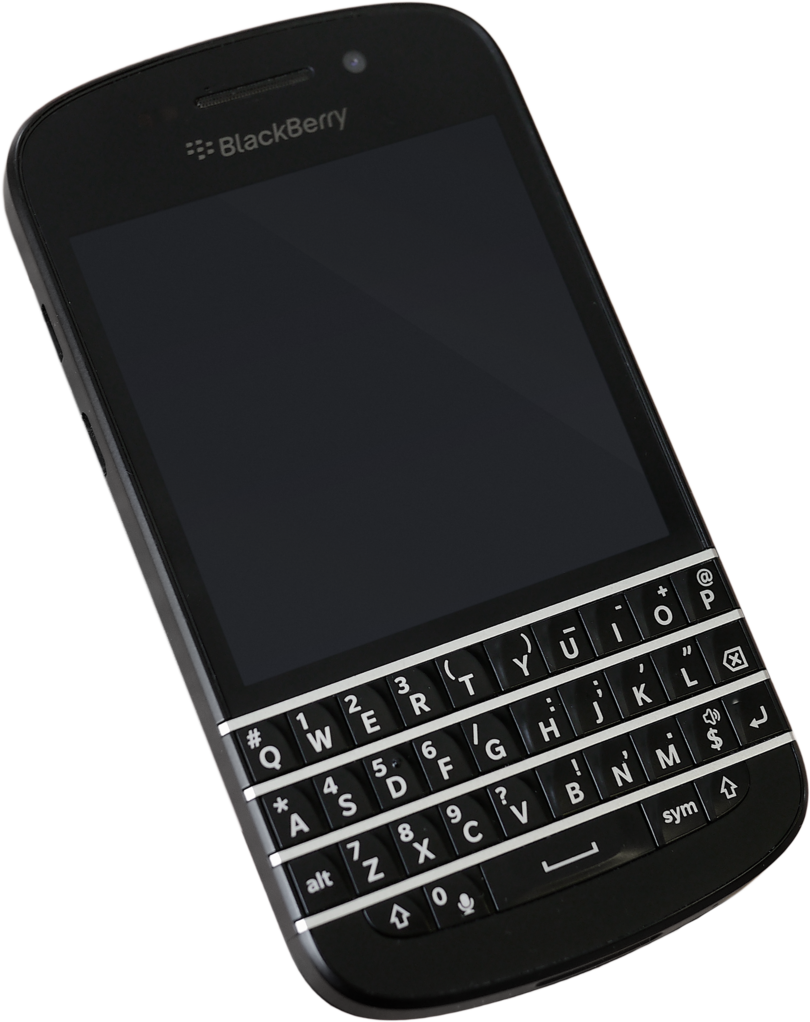
\includegraphics[width=0.4\textwidth]{../common/images/blackberry}
            }
        \end{column}
    \end{columns}

    \only<3->{
        \flushright
        \imagesource{https://en.wikipedia.org/wiki/File:Blackberry-Q10-transparent.png}
    }

    \notes {
        \item present pros and cons
        \item it's still the most common choice
        \item phones get smaller $\rightarrow$ deviceless
        \item \textbf{voice}: inaccurate, only nat. language, environment dependent
        \item \textbf{handwriting}: slow, touch screen, surface, inaccurate
        \item \textbf{visual methods}: very slow, good for handicapped users
    }
\end{frame}

\subsection{Vision}
\begin{frame}{Vision}
    \begin{enumerate}
        \item<1-> record finger movements and input while typing
        \item<2-> use machine learning for input prediction
        \item<3-> remove keyboard
        \item<4-> type everywhere
    \end{enumerate}

    \notes{
        \item simple to generate learning data
        \item complex movement we don't fully predict: (example with B key)
        \item \textbf{BUT FIRST!} let's see who did this already
    }
\end{frame}

\subsection{Related Work}
\begin{frame}{Related Work}{Sensor Gloves}
    \begin{itemize}
        \item gesture detection \citep{web:cyberglove} \citep{zimmerman-flex-gloves} \citep{imu-emg}
        \item sign language detection \citep{imu-emg} \cite{mehdi-sign-language-glove}
        \item music generation \citep{web:mimugloves}
        \item medical applications \citep{cavallo-senshand-parkinsons}
    \end{itemize}

    $\rightarrow$ overview at \citetitle{web:mimugloves-overview} \citep{web:mimugloves-overview}

    \notes{
        \item flex sensor gloves started 1987
    }
\end{frame}

\begin{frame}{Related Work}{Alternative Keyboard Inputs}
    \begin{itemize}
        \item buttons on glove \citep{web:keyglove}
        \item braille gloves \citep{braille-gloves}
        \item \citetitle{ellithorpe-kinect-typing} \citep{ellithorpe-kinect-typing} $\rightarrow$ Kinect
    \end{itemize}

    \centering
    \begin{figure}
        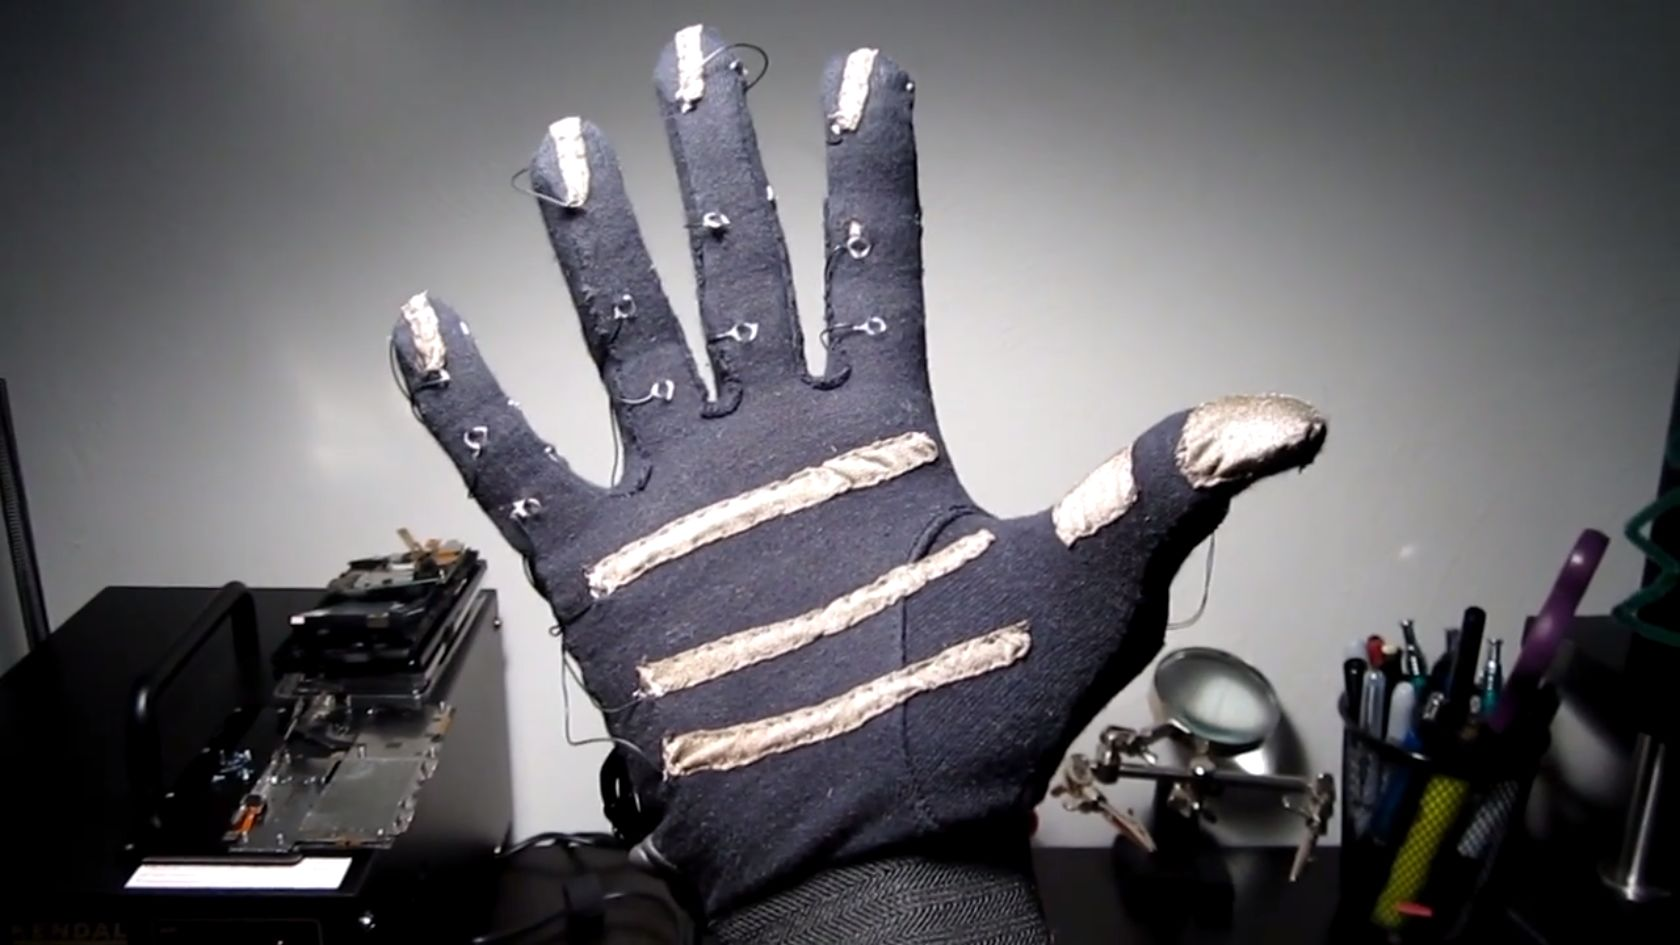
\includegraphics[width=0.55\textwidth]{../common/images/keyglove}
        \caption{The Keyglove - a wearable, wireless, open-source input device}
    \end{figure}
    \imagesource{https://vimeo.com/23269969}
\end{frame}

\begin{frame}{Related Work}{Commercial Products}
    \begin{itemize}
        \item \citetitle{web:gest} \citep{web:gest} {\scriptsize($\text{\$ }199,988$ on Kickstarter)}
        \item \citetitle{web:senseboard} \citep{web:senseboard}
        \item \citetitle{web:hi5vrglove} \citep{web:hi5vrglove} $\rightarrow$ VR Gaming
    \end{itemize}
    \begin{columns}[T]
        \begin{column}{0.48\textwidth}
            \begin{figure}
                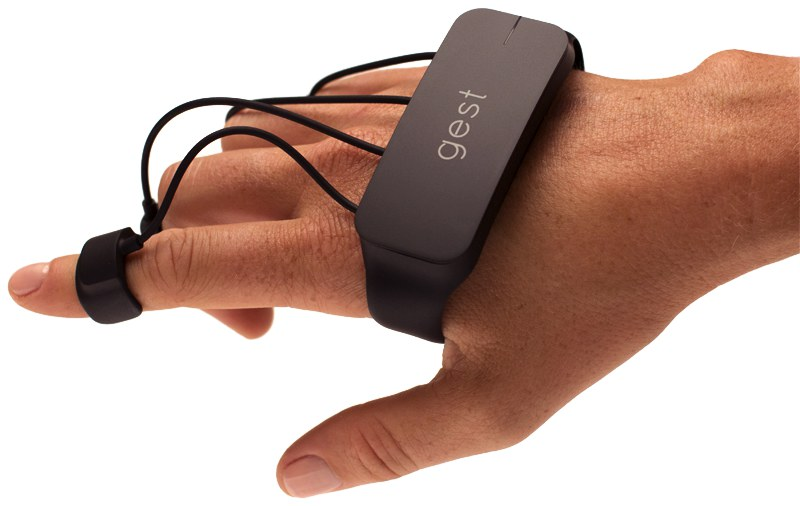
\includegraphics[height=3cm]{../common/images/gest}
                \imagesource{https://gest.co/}
                \caption{Gest general purpose interaction wearable}
            \end{figure}
        \end{column}
        \begin{column}{0.48\textwidth}
            \begin{figure}
                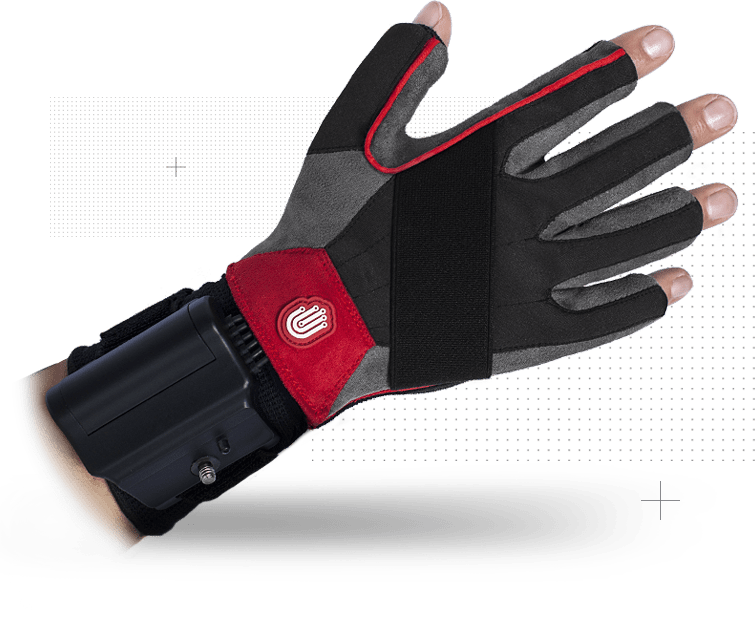
\includegraphics[height=3cm]{../common/images/hi5vr-glove}
                \imagesource{http://hi5vrglove.com/}
                \caption{Noitom Hi5 VR Glove}
            \end{figure}
        \end{column}
    \end{columns}

    \notes{
        \item \textbf{gest}
        \item raised \textasciitilde 200k USD on kickstarter in Oct 2015
        \item out of business within half a year, no funding
        \item \textbf{senseboard}
        \item weird project, no information available, no images
        \item same idea as we did
        \item \textbf{hi5vrglove}
        \item intended for VR gaming
        \item very new
        \item no typing software
        \item same hardware specs
        \item \textbf{gest at least advertised with keyboard functionality}
    }
\end{frame}

\begin{frame}{Related Work}{In Research}
    \center
    \vfill
    no research project combines\\[1em]
    sensor + keyboard data $\rightarrow$ machine learning
    \vfill
\end{frame}

\subsection{Project Goal}
\begin{frame}{Project Goal}
    Of course we won't build a fully working keyboard in 2 bachelor theses.
    \pause
    \vspace{2em}
    \begin{block}{Goal}
        Design a system for recording characteristic hand movements of typing
        and the corresponding input.\\[1em]

        Define an approach for utilizing machine learning to map the recorded
        data back to the keyboard input.\\[1em]

        Evaluate the quality of such mapping and discuss whether this principle
        could be turned into a working keyboard alternative.
    \end{block}
\end{frame}
